% Created 2022-04-28 Thu 11:41
% Intended LaTeX compiler: xelatex
\documentclass[letterpaper]{article}
\usepackage{graphicx}
\usepackage{longtable}
\usepackage{wrapfig}
\usepackage{rotating}
\usepackage[normalem]{ulem}
\usepackage{amsmath}
\usepackage{amssymb}
\usepackage{capt-of}
\usepackage{hyperref}
\usepackage[margin=1in]{geometry}
\setlength{\parindent}{0pt}
\usepackage[margin=1in]{geometry}
\usepackage{fontspec}
\usepackage{svg}
\usepackage{tikz}
\usepackage{cancel}
\usepackage{pgfplots}
\usepackage{indentfirst}
\setmainfont[ItalicFont = HelveticaNeue-Italic, BoldFont = HelveticaNeue-Bold, BoldItalicFont = HelveticaNeue-BoldItalic]{HelveticaNeue}
\newfontfamily\NHLight[ItalicFont = HelveticaNeue-LightItalic, BoldFont       = HelveticaNeue-UltraLight, BoldItalicFont = HelveticaNeue-UltraLightItalic]{HelveticaNeue-Light}
\newcommand\textrmlf[1]{{\NHLight#1}}
\newcommand\textitlf[1]{{\NHLight\itshape#1}}
\let\textbflf\textrm
\newcommand\textulf[1]{{\NHLight\bfseries#1}}
\newcommand\textuitlf[1]{{\NHLight\bfseries\itshape#1}}
\usepackage{fancyhdr}
\usepackage{csquotes}
\pagestyle{fancy}
\usepackage{titlesec}
\usepackage{titling}
\makeatletter
\lhead{\textbf{\@title}}
\makeatother
\rhead{\textrmlf{Written} \today}
\lfoot{\theauthor\ \textbullet \ \textbf{2021-2022}}
\cfoot{}
\rfoot{\textrmlf{Page} \thepage}
\renewcommand{\tableofcontents}{}
\titleformat{\section} {\Large} {\textrmlf{\thesection} {|}} {0.3em} {\textbf}
\titleformat{\subsection} {\large} {\textrmlf{\thesubsection} {|}} {0.2em} {\textbf}
\titleformat{\subsubsection} {\large} {\textrmlf{\thesubsubsection} {|}} {0.1em} {\textbf}
\setlength{\parskip}{0.45em}
\renewcommand\maketitle{}
\author{Houjun Liu}
\date{\today}
\title{MVC 2 PS\#25}
\hypersetup{
 pdfauthor={Houjun Liu},
 pdftitle={MVC 2 PS\#25},
 pdfkeywords={},
 pdfsubject={},
 pdfcreator={Emacs 28.0.91 (Org mode 9.5.2)}, 
 pdflang={English}}
\begin{document}

\maketitle
\tableofcontents

We do the problems again, but corrected!

\section{Single Value Function}
\label{sec:orga7f1c1e}
\begin{quote}
\begin{align}
   &f_1: \mathbb{R}^2 \to \mathbb{R}^1 \\ 
&f_1(x,y) = 0
\end{align}

What's the area of this function?
\end{quote}

\begin{verbatim}
f(x,y) = 0
plot3d(f, (x,0,5), (y,0,7))
\end{verbatim}

\begin{center}
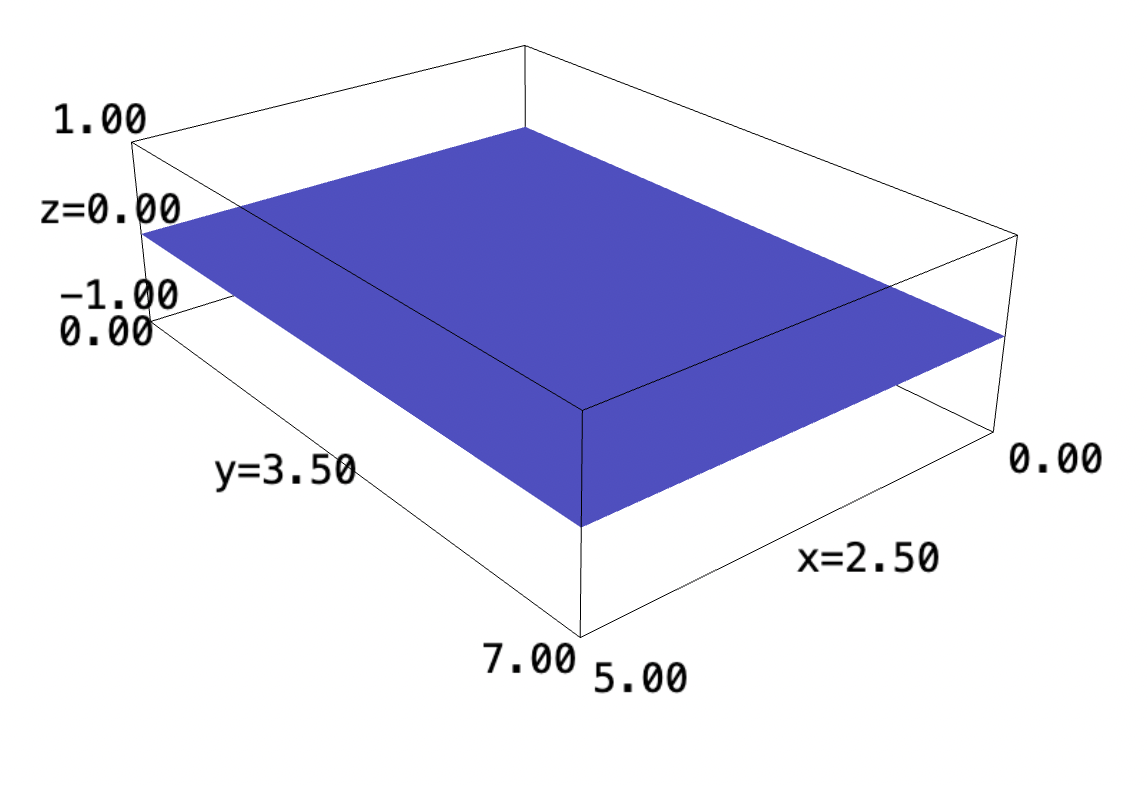
\includegraphics[width=.9\linewidth]{2022-04-25_09-53-13_screenshot.png}
\end{center}

We can take the area of the shape, essentially by taking the volume by height \(1\): that is, for a rectangle of \(l,w,h\), its top-area is simply \(l\cdot w\), also known as \(lw\cdot 1\). Therefore:

\begin{equation}
   \int_0^7 \int_0^5 1 dx\ dy = 35
\end{equation}

The area of the shape is therefore \(35\).

\section{Area of the Plane}
\label{sec:orge59cadc}
We want to first figure the correction per every given slice \(dA=n\ dV\) to setup a surface integral. By pythagoras (i.e. projecting the changes to the parallelity of the surface), we have that:

\begin{equation}
   dA = \sqrt{1+\left(\frac{\partial f}{\partial x}\right)^2+\left(\frac{\partial f}{\partial y}\right)^2}\ dV
\end{equation}

\begin{quote}
What's the area of the following function by \((5,7)\)?

\begin{align}
   &f_2: \mathbb{R}^2 \to \mathbb{R}^1 \\ 
&f_2(x,y) = 2x+3y+10
\end{align}
\end{quote}

\begin{verbatim}
f(x,y) = 2*x+3*y+10
plot3d(f, (x,0,5), (y,0,7))
\end{verbatim}

\begin{center}
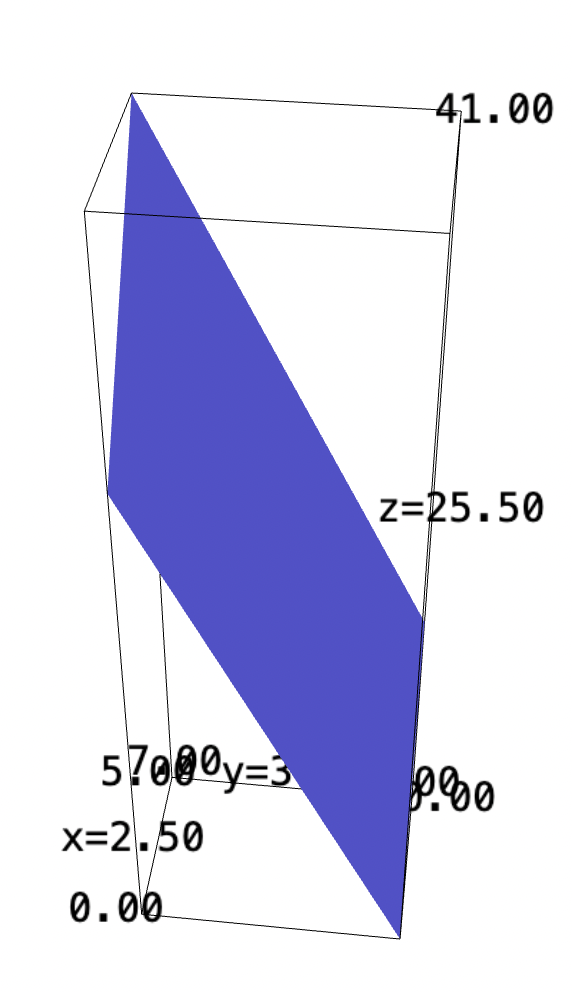
\includegraphics[width=.9\linewidth]{2022-04-25_09-53-43_screenshot.png}
\end{center}

\begin{equation}
   dA = \sqrt{1+4+9} dV = \sqrt{14}\ dV
\end{equation}

Therefore, taking the integral:

\begin{align}
   &\int_0^5 \int_0^7 \sqrt{14}\ dy\ dx \\
\Rightarrow & 35\sqrt{14}
\end{align}

\begin{verbatim}
float(35*sqrt(14))
\end{verbatim}

\begin{verbatim}
130.95800853708795
\end{verbatim}


It appears that the surface area is about \(130.958\) units.

\section{Area of a Parabola}
\label{sec:org212a7c6}
\begin{quote}
What's the area of the following function by \((5,7)\)?

\begin{align}
   &f_3: \mathbb{R}^2 \to \mathbb{R}^1 \\ 
&f_3(x,y) = x^2
\end{align}
\end{quote}

\begin{verbatim}
f(x,y) = x^2
plot3d(f, (x,0,5), (y,0,7))
\end{verbatim}

\begin{center}
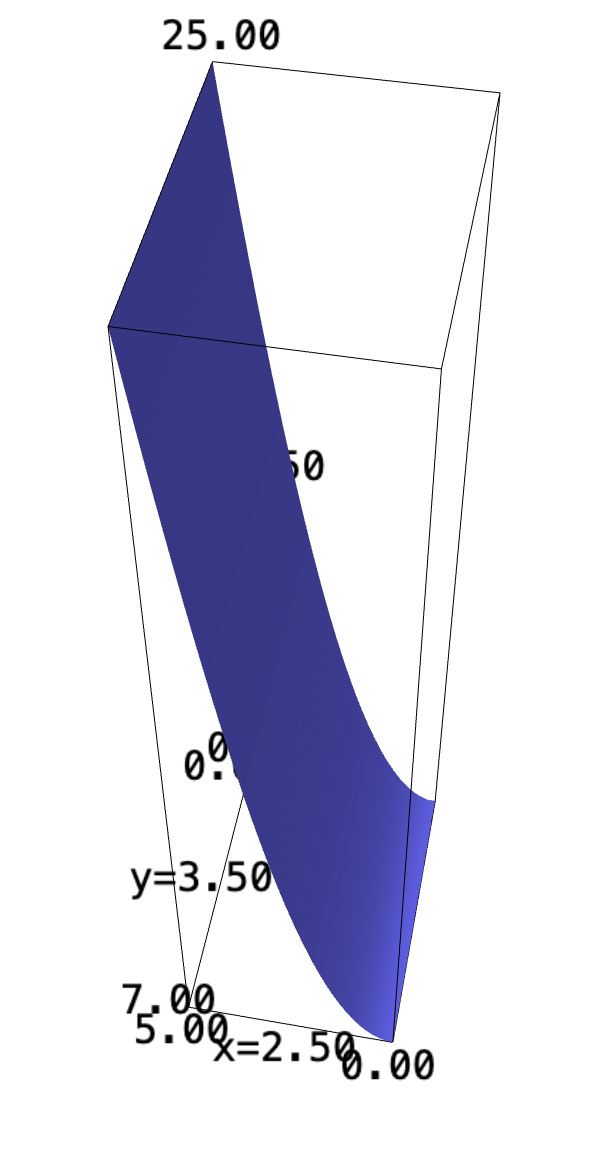
\includegraphics[width=.9\linewidth]{2022-04-25_09-54-21_screenshot.png}
\end{center}


We will again find the area correction factor:

\begin{equation}
   dA = \sqrt{1+4x^2}\ dV
\end{equation}

And therefore, taking the integral:

\begin{equation}
  \int_0^5 \int_0^7 \sqrt{1+4x^2}\ dy\ dx
\end{equation}

This problem is solvable by trig substitution followed by integration by parts. For now, however, we will leverage a calculator.

\begin{verbatim}
f(x,y) = sqrt(1+4*x^2)
f.integrate(y, 0,7).integrate(x,0,5)
float(f.integrate(y, 0,7).integrate(x,0,5))
\end{verbatim}

\begin{verbatim}
35/2*sqrt(101) + 7/4*arcsinh(10)
181.119713532637
\end{verbatim}


Evidently, the surface area of the shape is about \(181.1197\) units.

\section{Another Surface Area}
\label{sec:org82191af}
\begin{quote}
What's the area of the following function by \((5,7)\)?

\begin{align}
   &f_3: \mathbb{R}^2 \to \mathbb{R}^1 \\ 
&f_3(x,y) = x^2-y^2
\end{align}
\end{quote}

\begin{verbatim}
f(x,y) = (x^2-y^2)*sqrt(1+4*x^2+4*y^2)
plot3d(f, (x,0,5), (y,0,7))
\end{verbatim}

\begin{center}
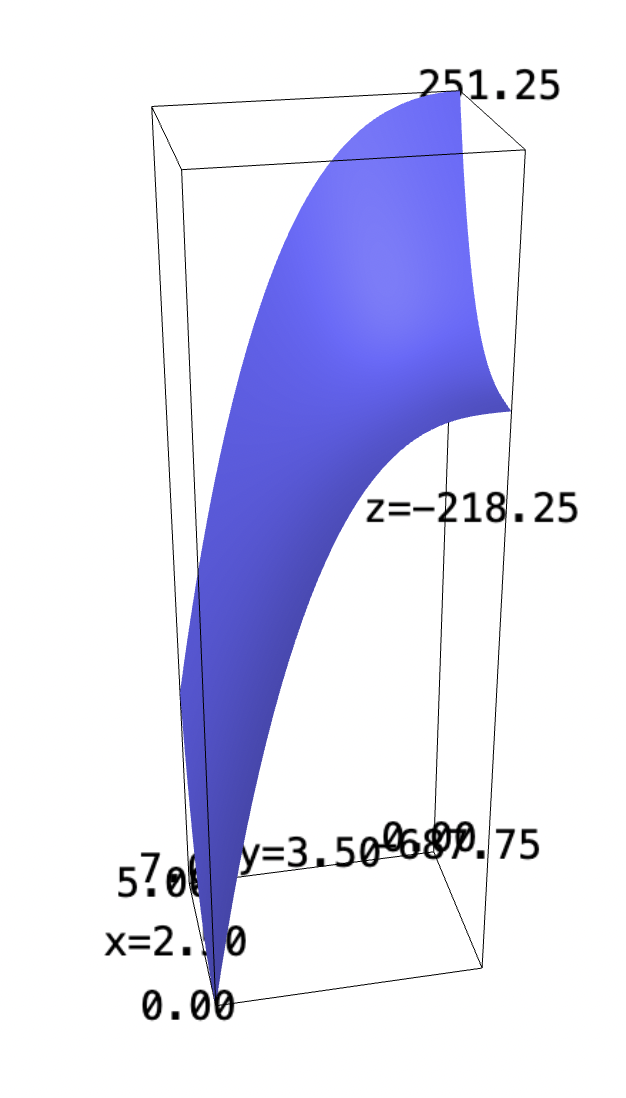
\includegraphics[width=.9\linewidth]{2022-04-25_09-54-54_screenshot.png}
\end{center}

Let's instead parameterize this function first to take its surface area. We will take the most basic parameterization.

\begin{equation}
\vec{v}(x,y) = x \hat{i} + y \hat{j} + (x^2-y^2) \hat{k} 
\end{equation}

Taking, therefore, the partial derivatives:

\begin{align}
   &\frac{\partial \vec{v}}{\partial x} = \hat{i} + 2x \hat{k}\\
   &\frac{\partial \vec{v}}{\partial y} = \hat{j} - 2y \hat{k}
\end{align}

Taking their cross product for the differential area, then:

\begin{align}
& (\hat{i} + 2x \hat{k}) \times (\hat{j} - 2y \hat{k})\\
\Rightarrow & (\hat{i}\hat{j} + 2x \hat{k}\hat{j} - \hat{i}2y \hat{k} -2x \hat{k}2y \hat{k})\\
\Rightarrow & (\hat{k} - 2x \hat{i} + 2y \hat{j})
\end{align}

We will take now the magnitude of this expression:

\begin{equation}
   \sqrt{1^2 + (-2x)^2 + (2y) ^2 } = \sqrt{1 + 4x^2 + 4y^2}
\end{equation}

We will again take this integral, digitally this time:

\begin{equation}
  \int_0^5 \int_0^7 \sqrt{1+4x^2+4y^2} \ dy\ dx
\end{equation}

\begin{verbatim}
f(x,y) = sqrt(1+4*x^2+4*y^2)
f.integrate(y, 0,7).integrate(x,0,5)
float(f.integrate(y, 0,7).integrate(x,0,5))
\end{verbatim}

\begin{verbatim}
35*sqrt(33) - 1/12*arctan(1/14) + 1/12*arctan(-15/7*sqrt(33) + 101/14) + 1393/24*log(197) + 515/12*log(1/101*sqrt(101)*(3*sqrt(101)*sqrt(33/101) + 14)) - 1393/12*log(3*sqrt(33) - 10)
326.54996642727804
\end{verbatim}


The shape is largely underneath the x-axis during the area on the rectangle. Therefore, we have an negative area! It is about \(326.55\) units.
\end{document}